\section{Search Metrics}
\label{app:search_metrics}
Here, we detail the computation of each metric shown in Fig.\ref{fig:search}.
For an idea $\boldsymbol{\mathcal{I}}$, let $\boldsymbol{\mathcal{R}}$ denote the set of all resources retrieved by a method, and $\boldsymbol{\mathcal{R}}_h\subseteq \boldsymbol{\mathcal{R}}$ the subset of highly relevant resources.
Let $\boldsymbol{\mathcal{T}}_{\boldsymbol{\mathcal{I}}}$ be the main topic words contained in idea $\boldsymbol{\mathcal{I}}$, and $\boldsymbol{\mathcal{T}}_{r_i}$ the main topic words contained in each resource $r_i\in \boldsymbol{\mathcal{R}}, 1 \leq i \leq |\boldsymbol{\mathcal{R}}|$.
The metrics are then defined as follows:
\begin{itemize}[topsep=0pt,partopsep=0pt,parsep=0pt,itemsep=0pt,leftmargin=*,labelsep=0.5em]
    \item \textbf{Relevance Density.}
    This metric quantifies the relevance degree of retrieved resources. We use an LLM to determine highly relevant sources $\boldsymbol{\mathcal{R}}_h$ returned by each method. To prevent methods from winning simply by retrieving more total items, we divide the count of highly relevant resources $|\boldsymbol{\mathcal{R}}_h|$ by the total number retrieved $|\boldsymbol{\mathcal{R}}|$, yielding the relevance density of each search strategy:
    \begin{align}
        \textbf{Relevance Density} = \frac{|\boldsymbol{\mathcal{R}}_h|}{|\boldsymbol{\mathcal{R}}|}.
    \end{align}
    \item \textbf{Topic Coverage.} This metric measures the comprehensiveness of the retrieved resources, specifically the extent to which the topic keywords covered by the retrieved resources overlap with those of the idea. It is defined as follows:
    \begin{align}
        \textbf{Topic Coverage} = \frac{|\boldsymbol{\mathcal{T}}_{\boldsymbol{\mathcal{I}}}\cap(\boldsymbol{\mathcal{T}}_{r_1}\cup\dots\cup\boldsymbol{\mathcal{T}}_{r_{|\boldsymbol{\mathcal{R}}|}})|}{|\boldsymbol{\mathcal{T}}_{\boldsymbol{\mathcal{I}}}|}
    \end{align}
    \item \textbf{Diversity.} This metric quantifies the diversity of the retrieved resources, expressed as the proportion of topic keywords beyond those already covered in the idea that appear in the retrieved documents:
    \begin{align}
        \textbf{Diversity} = \frac{|\boldsymbol{\mathcal{T}}_{r_1}\cup\dots\cup\boldsymbol{\mathcal{T}}_{r_{|\boldsymbol{\mathcal{R}}|}}-\boldsymbol{\mathcal{T}}_{\boldsymbol{\mathcal{I}}}|}{|\boldsymbol{\mathcal{T}}_{r_1}\cup\dots\cup\boldsymbol{\mathcal{T}}_{r_{|\boldsymbol{\mathcal{R}}|}}|}
    \end{align}
    \item \textbf{Quality.} We directly employ an LLM to assess the quality of each retrieved resource and assign it a score $s_{r_i}$. The final metric is the average quality across all resources:
    \begin{align}
        \textbf{Quality} = \frac{\sum_{i=1}^{|\boldsymbol{\mathcal{R}}|}s_{r_i}}{|\boldsymbol{\mathcal{R}}|}
    \end{align}
\end{itemize}
All LLMs employed in the above computations are DeepSeek-V3.2.

\begin{figure*}
    \centering
    % \vspace{-1.1cm}
    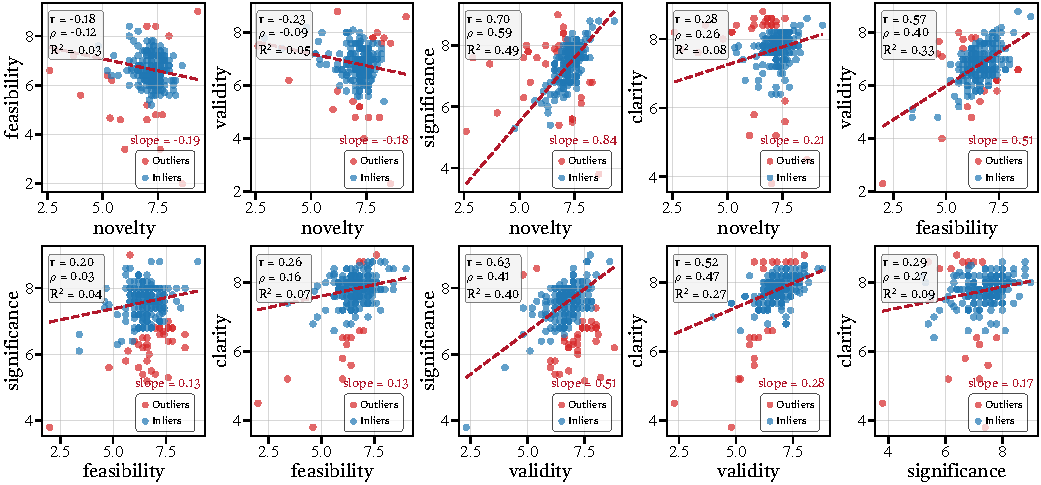
\includegraphics[width=1.\textwidth]{figure/all_pairs.pdf}
    % \vspace{-0.5cm}
    \caption{\textbf{Scatter Plots Between Metric Pairs.} We perform linear regression fitting for each metric pair. The red dashed line is the fit after removing outliers, and its \textit{slope} is reported. $r$ denotes the Pearson coefficient, $\rho$ is the Spearman coefficient, and R$^2$ represents the fit goodness of all inliers explained by the fitted line.}
    \label{fig:all_metrics_pair}
    \vskip -0.2in
\end{figure*}